\subsection{Hip\'otesis}
	Con los experimentos se busca comprobar las siguientes hipotesis:\\
	1. Hacer un sort de los elementos de mayor a menor, hace que las podas sean m\'as efectivas.\\
	2. Hacer un sort de los elementos de menor a mayor, hace que las podas empeoren.\\
	3. La podas podas empeora a medida que el valor de los elementos se acercan a 0, y mejora a medida que el valor de los elementos se acercan al valor objetivo.\\
	4. Fuerza Bruta depende únicamente de la cantidad de items.\\
	5. Las podas de factibilidad y optimalidad en mejor caso tienen complejidad lineal.\\
\subsection{Consideraciones para las experimentaciones}
\subsubsection{Generaci\'on de elementos}
\begin{itemize}
	\item Se usa la función sort de c++ (ordena los elementos en forma creciente)
	\item Los conjuntos fueron generados aleatoriamente, con la funci\'on rand de c++ (distribución uniforme) para poder analizar en caso promedio que pasaba con cada algoritmo, en el rango entre [0..$V$].
	\item la cantidad de iteraciones es igual a 50, pues se logro ver durante la experimentaci\'on que los algoritmos se estabilizaban.
	\item El rango para la suma fue [15000...800000], porque es limitada por Programación Dinámica, la cual pide memoria de tamaño $n*W$ y al ser $W$ tan grande, hace que no se pueda seguir experimentando.
	\item El rango para la cantidad de elementos fue [5...35], porque al querer analizar el caso promedio se toma el promedio de 50 iteraciones y los algoritmos exponenciales tardan demasiado.
\end{itemize}
\subsubsection{Im\'agenes}
\begin{itemize}
	\item La etiqueta $decreciente$ indica que los elementos fueron ordenados de menor a mayor para hacer la experimentaci\'on.
	\item La etiqueta $creciente$ indica que los elementos fueron ordenados de menor a mayor para hacer la experimentaci\'on.
	\item La etiqueta $unSort$ indica que los elementos no fueron ordenados.
\end{itemize}	
\subsection{Complejidades Te\'oricas en la pr\'actica}
\subsubsection{Fuerza Bruta}
La Figura 1 muestra como Fuerza Bruta no es afectada por el sort de los elemento, y al aplicarle el logaritmo en base dos se logra ver que es lineal, lo cual es esperado pues es exponencial en la cantidad de elementos con base igual a 2.
\begin{figure}[h]
\centering
	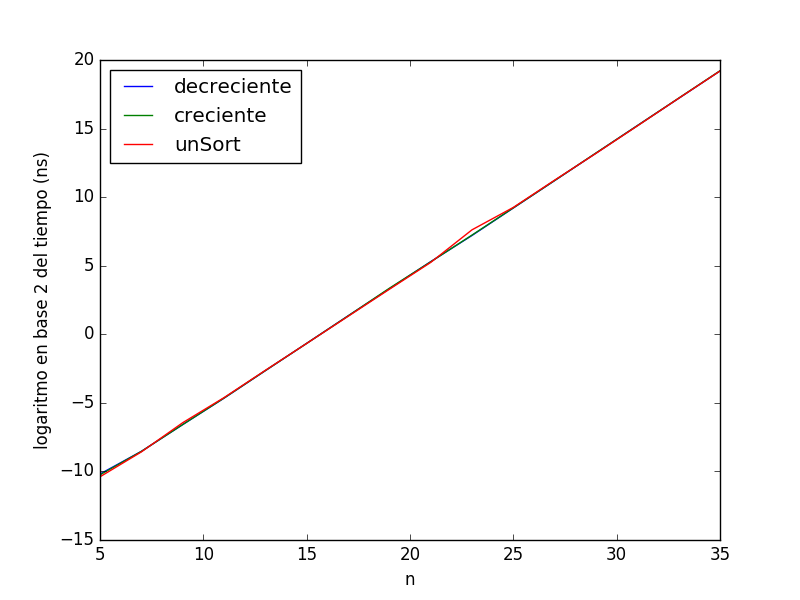
\includegraphics[width=0.6\textwidth]{fbSort.png}
\caption{Relación entre el orden de los elementos y la complejidad temporal}
\end{figure}

\subsubsection{Backtracking poda por factibilidad}
Tener los elementos ordenados de mayor a menor hace que la poda sea mas efectiva pues al considerar los elementos de mayor valor primero el algoritmo se ahorra comparaciones y empeora cuando el ordenamiento es de menor a mayor.\\ 
Por ejemplo: $Conj1 = \{1,2\}$, $Conj2 = \{2,1\}$ y el valor objetivo 2. \\
Para el $Conj1$, considera los subconjuntos $\{ 1\}$, $\{ 1,2\}$, y $\{2\}$.\\
Para el $Conj2$, considera los subconjuntos $\{2\}$ pues no necesita agregar nada mas para llegar al valor objetivo y $\{1\}$.\\
El algoritmo hace una comparación menos, pero si el conjunto es mas grande podría hacer menos comparaciones si la suma de los elementos exceden el valor objetivo.\\
Se aplica logaritmo en base dos y se logra ver que el resultado es lineal.\\
Los picos de la función se deben a las podas realizadas.\\
\begin{figure}[h]
\centering
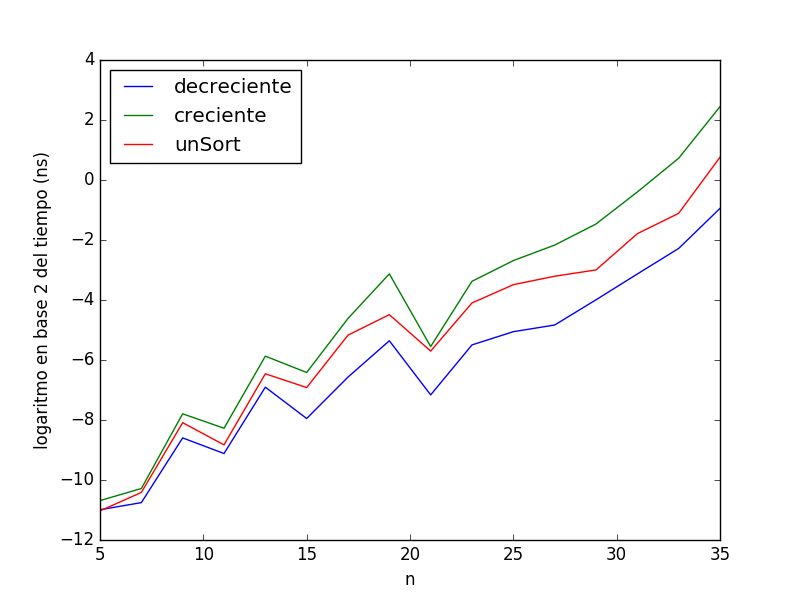
\includegraphics[width=0.6\textwidth]{facSort.png}
\caption{Relación entre el orden de los elementos y la complejidad temporal}
\end{figure}

\subsubsection{Backtracking poda por optimalidad}
El ordenamiento de los elementos afecta a la poda de optimalidad.\\
Por ejemplo: $Conj1 = \{3,4\}$, $Conj2 = \{4,3\}$ y el valor objetivo 4. \\
Para el $Conj1$, considera los subconjuntos $\{ 3\}$, $\{ 3,4\}$, y $\{4\}$.\\
Para el $Conj2$, considera los subconjuntos $\{4\}$ por que la suma del primer subconjunto es el valor objetivo y el cardinal óptimo es 1, entonces no considera conjuntos mayores o iguales a 1\\
\begin{figure}[h]
\centering
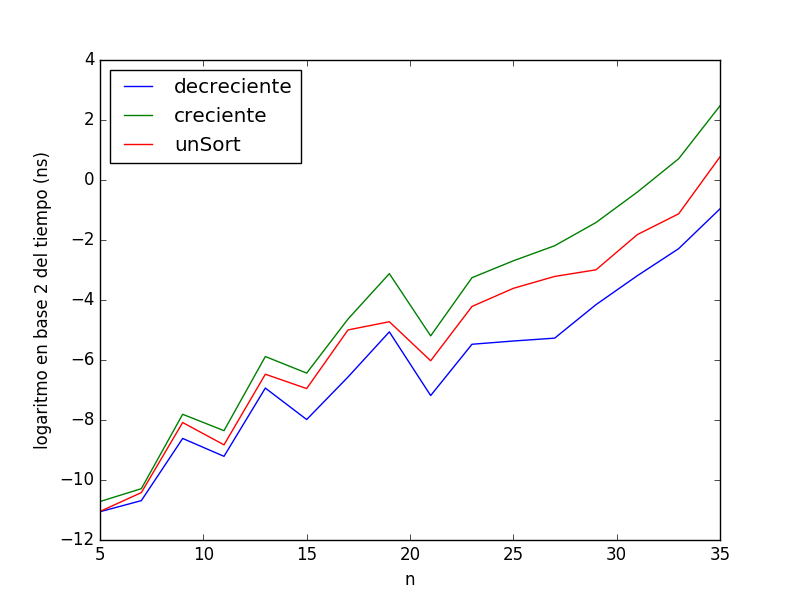
\includegraphics[width=0.6\textwidth]{opSort.png}
\caption{Relación entre el orden de los elementos y la complejidad temporal}
\end{figure}

\subsubsection{Programación dinámica}
En este experimento se fija $n=35$ y se varia $V$ para ver como afecta a la complejidad temporal.\\
En la figura 4 se ve como Programacion Dinamica es afectado directamente por el valor objetivo y en menor medida por el ordenamiento de los elementos.
\begin{figure}[h]
\centering
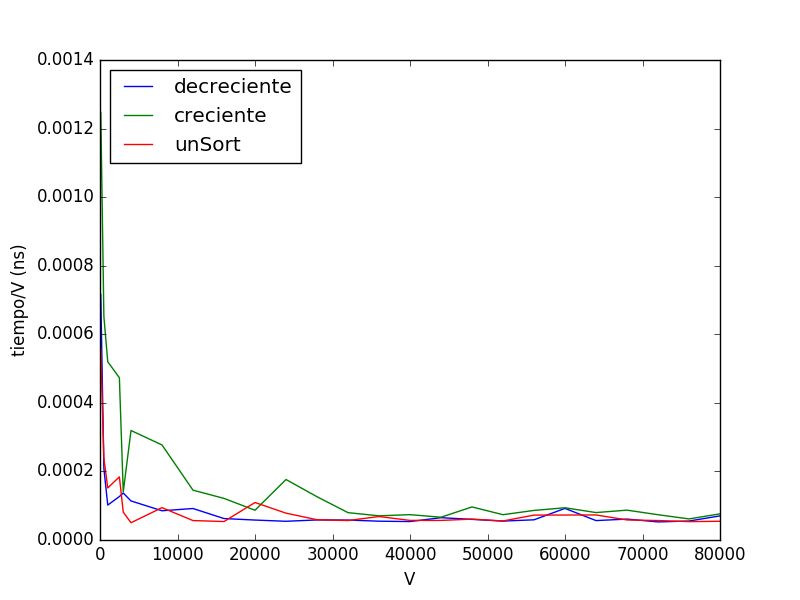
\includegraphics[width=0.6\textwidth]{pdObjetivo.png}
\caption{Relación entre el orden de los elementos, el valor objetivo y la complejidad temporal}
\end{figure}

\subsubsection{Influencia del valor de los elementos}
Para este experimento se fija $V=800000$ y $n=25$.\\
En la figura 5 el valor de los elementos se genera entre $[0,...,V/i]$ para la posición i.\\
Se logra ver que a medida que los elementos decrecen las podas no son tan efectivas.\\
Fuerza Bruta no es afectado por el valor de los elementos.\\
Programaci\'on dinámica es menos afectada por el decrecimiento del valor de los elementos.\\
\begin{figure}[h]
\centering
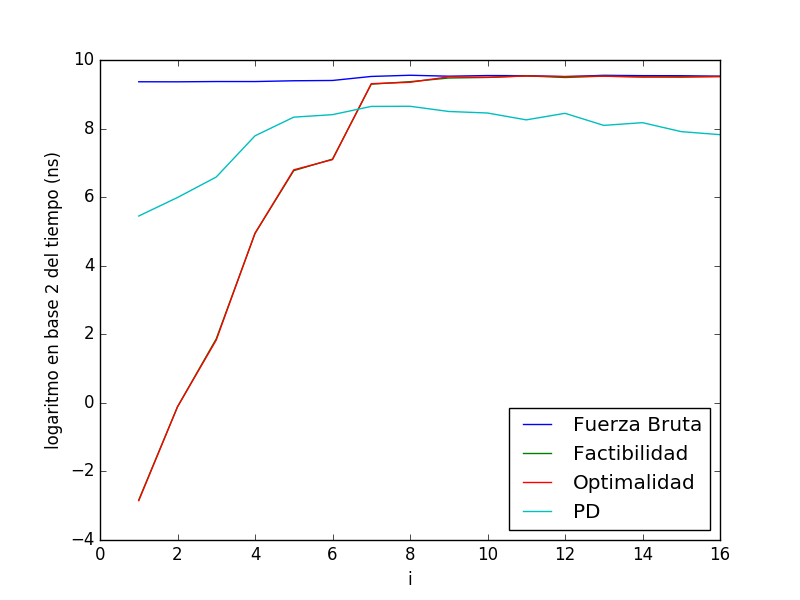
\includegraphics[width=0.6\textwidth]{todostodos.png}
\caption{Relación entre el decrecimiento de el valor de los elementos y como afecta a las complejidades}
\end{figure}\\
Este caso fue generado para ver el comportamiento lineal de estos algoritmos en mejor caso.\\
Los elementos son exactamente el valor objetivo y a medida que va creciendo la cantidad de elementos la complejidad temporal dividida por la cantidad de elementos se ajusta mejor.
\begin{figure}[h]
\centering
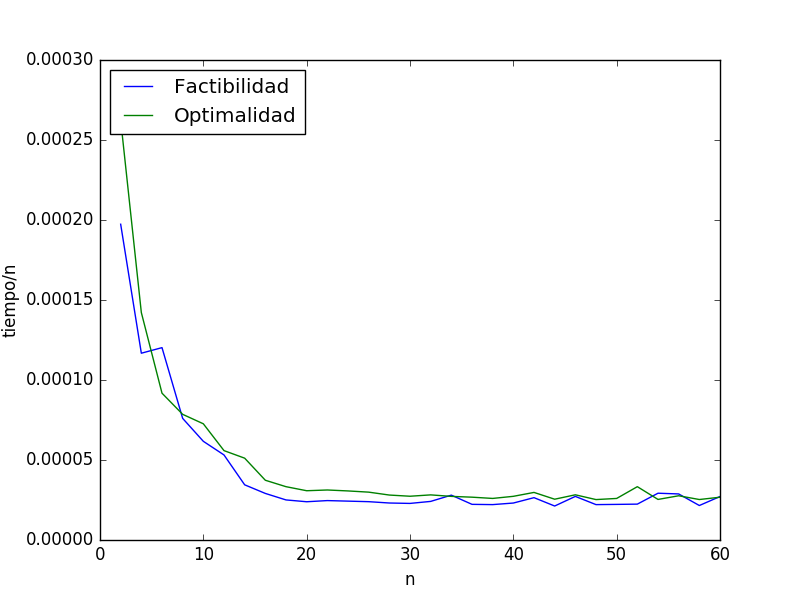
\includegraphics[width=0.6\textwidth]{mejorcasoBack.png}
\caption{Mejor caso para las podas, tiempo lineal}
\end{figure}